
\subsection{Initial density estimation}

The impinging $\alpha$-particles create free charge carriers within a small volume of the diamond bulk. 
The ionisation volume is described by the penetration depth of the $\alpha$-particle and its radial size. 
An average penetration depth of $\dpen \approx \SI{10}{\micro\meter}$ is calculated making use of NIST data
 and the radial $1/e$ size is estimated to be $r_0 \approx \SI{2}{\nm}$. 
The short $r_0$ is a result of the amount of energy transferred from the primary $\alpha$-particle to the electrons, 
 which is of the order of 60\,eV, cf.\ \cite{JansenThesis}, section 3.1.1. 
The aspect ratio of the ionisation volume is roughly $\num{10000}/\num{2} = \num{5000}$. 
As is shown later, the amount of charge produced at room temperature is about $Q = \SI{52}{\femto\coulomb}$,
 matching an estimate of an $\alpha$-particle with $\SI{4.3}{\mega\eV}$ at an electron-hole-pair creation energy of $\SI{13.25}{\eV}$. 
The average charge density in the first radial $1/e$ length of the charge cloud in the instant of the impingement is hence estimated as 

\begin{equation}
 n = \frac{0.68\cdot\SI{52}{\femto\coulomb}}{r_0^2\pi \dpen} \approx \SI{5e21}{\pairs/\cm^{3}}.
\end{equation}

\subsection{Induced current pulses from carrier drift}
\begin{figure}[tb]
 \centering
 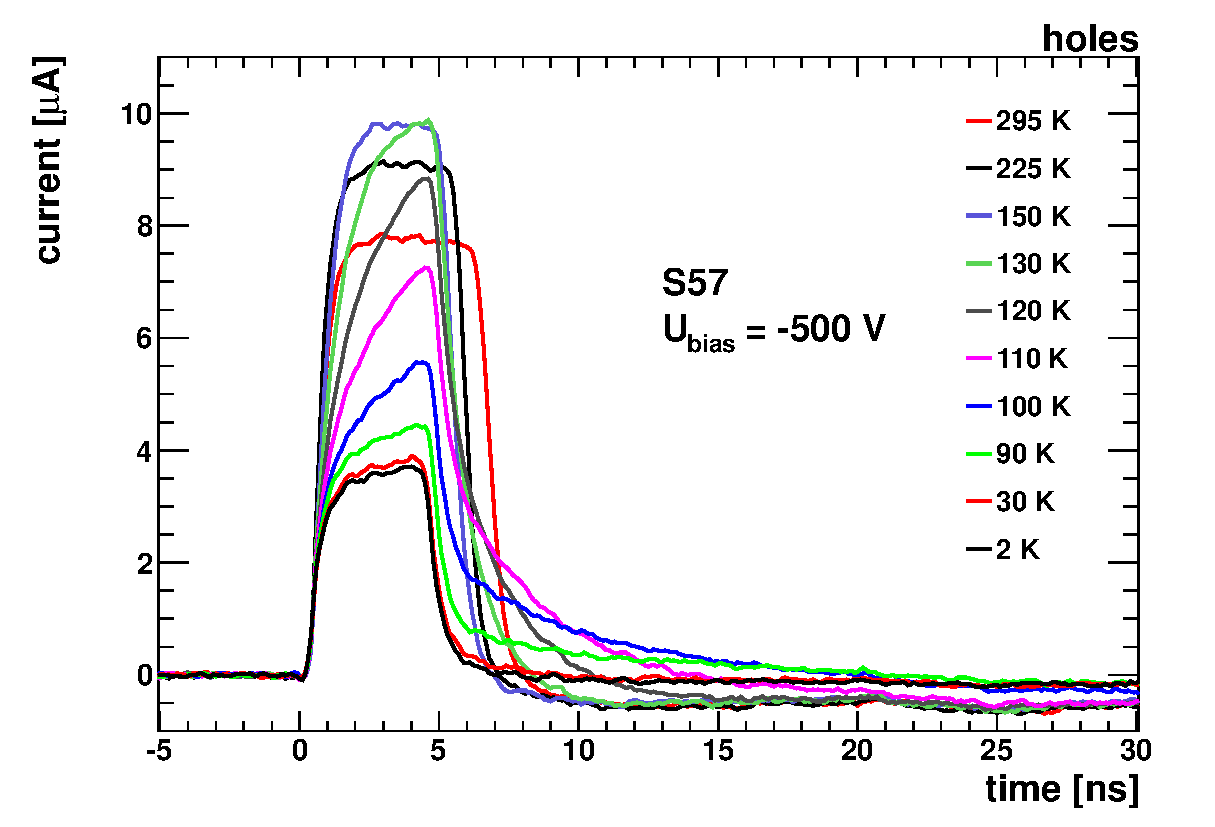
\includegraphics[width=0.49\textwidth]{figures/TCTholes500_exS57.eps}
 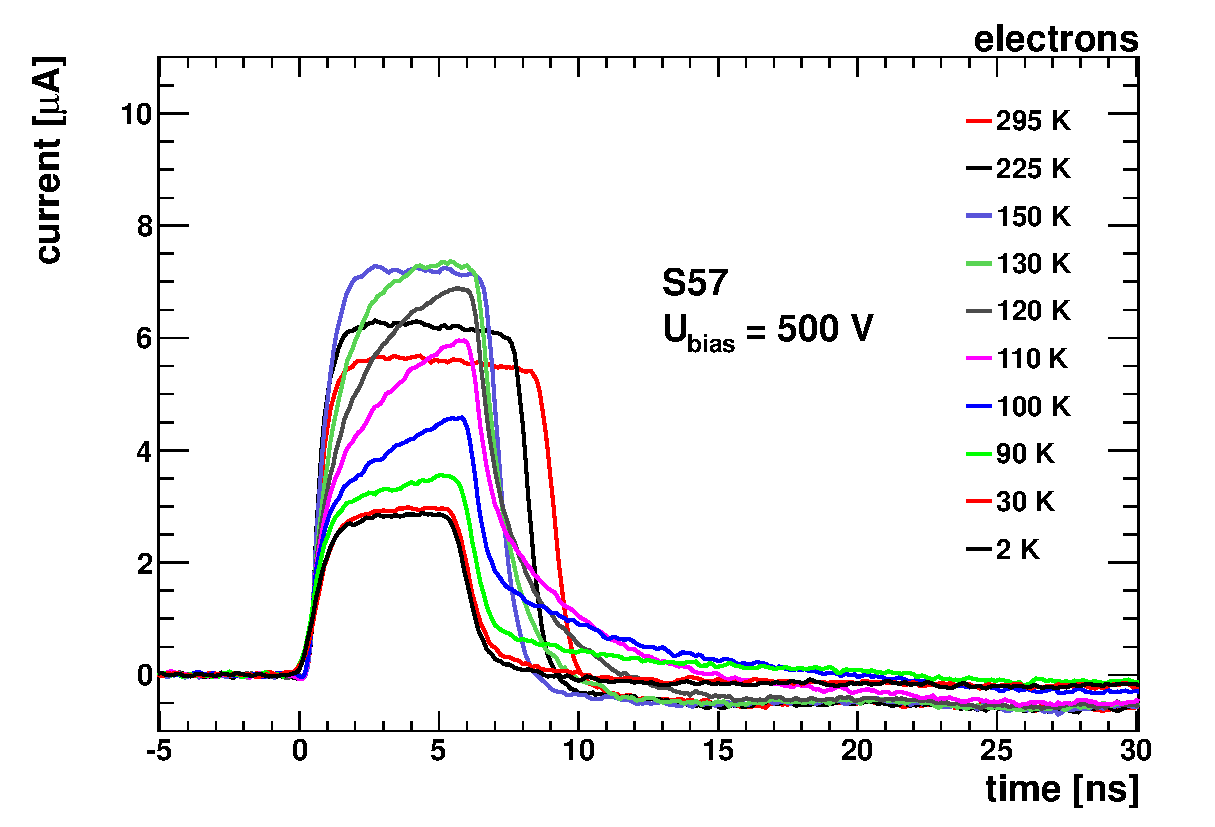
\includegraphics[width=0.49\textwidth]{figures/TCTelecs500_exS57.eps}
 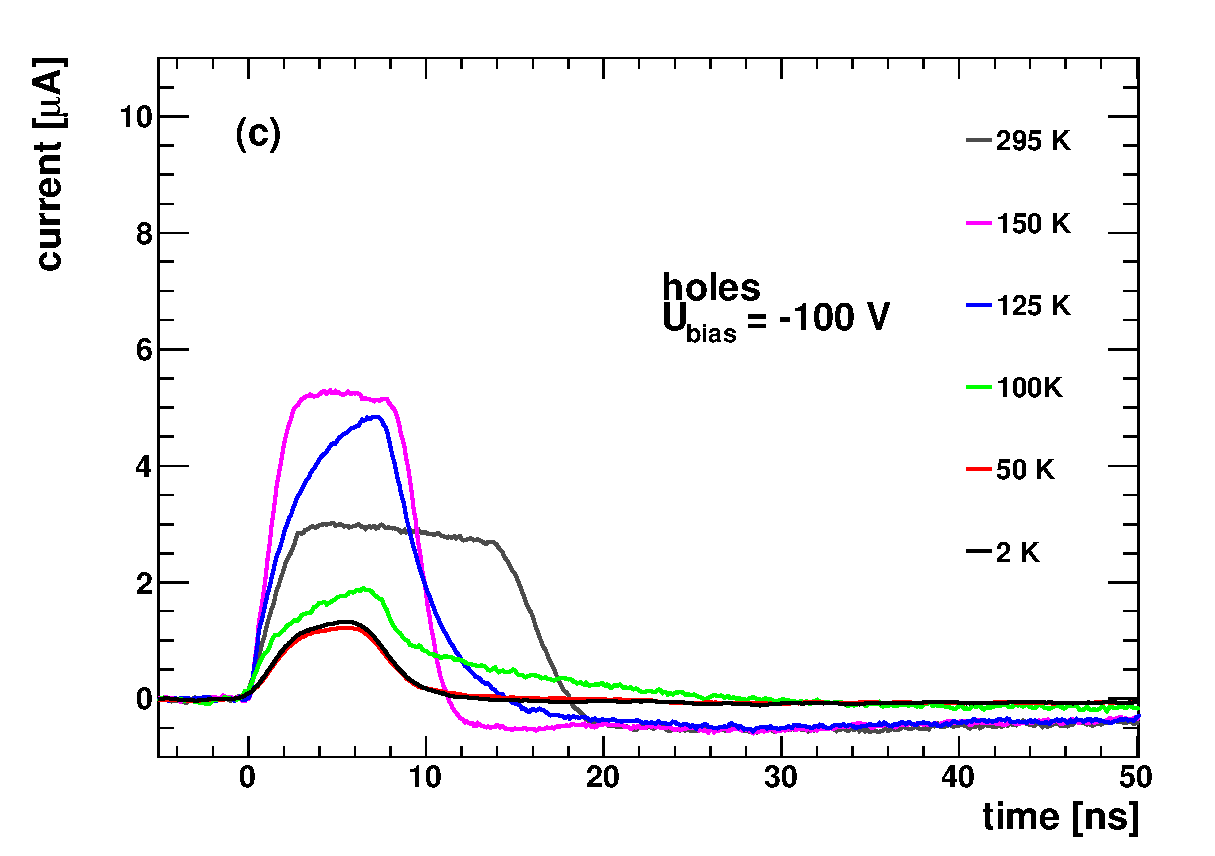
\includegraphics[width=0.49\textwidth]{figures/TCTholes100.eps}
 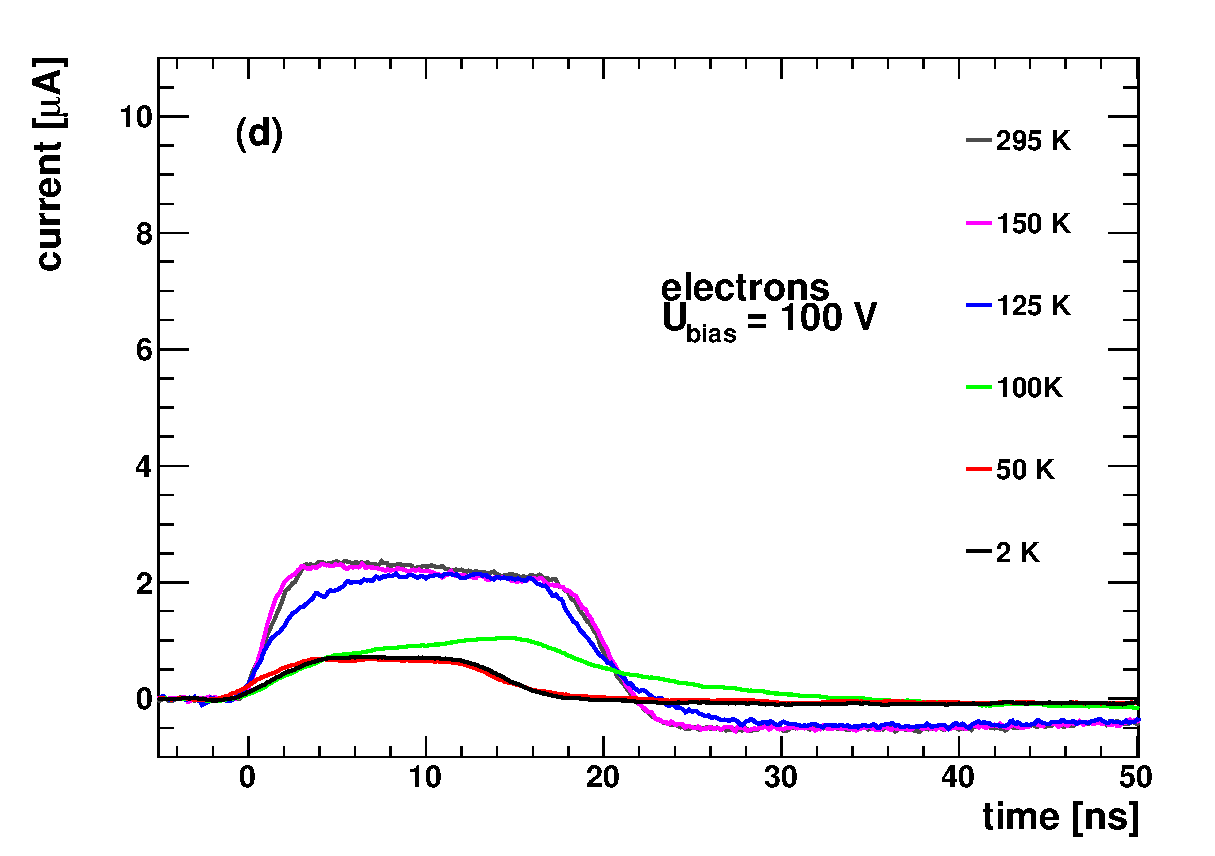
\includegraphics[width=0.49\textwidth]{figures/TCTelecs100.eps}

 \caption{Averaged current pulses for holes \textbf{(left column)} and electrons \textbf{(right column)} at various temperatures for
 $U_{\textrm{bias}} = \pm\SI{500}{\volt}$ \textbf{(top row)} and $U_{\textrm{bias}} = \pm\SI{100}{\volt}$ \textbf{(bottom row)} are shown for \textit{S57}.
 Note the similarity of electron pulses at $\SI{150}{\kelvin}$ and $\SI{295}{\kelvin}$. 
 Pulses from \textit{S52} and \textit{S79} are very similar and hence omitted.}
 \label{fig:currentprofiles}
\end{figure}

Hole and electron induced currents were recorded for temperatures between $T$ = 295\,K and  $\SI{2}{\kelvin}$. 
The set bias voltages covered a range from $ \SI{30}{\volt} \leq |V_{\textrm{bias}}| \leq \SI{900}{\volt}$ corresponding to electric field strengths from $\SI{0.06}{\volt/\um}$ to $\SI{1.8}{\volt/\um}$. 
Figure~\ref{fig:currentprofiles} shows a selection of the recorded and averaged pulses for SUT \textit{S57} at $\SI{\pm 500}{\volt}$ (top row) and $\SI{\pm 100}{\volt}$ (bottom row) for holes (left column)
 and electrons (right column). 
The electrons pulses are shown with an inverted current sign. 
Additional current pulses for samples \textit{S52} and \textit{S79} are published in \cite{JansenThesis}. 
At $\SI{\pm 500}{\volt}$, fast rise-times ($t_{\textrm{rise}} < \SI{1}{\nano\second}$) to about $\SI{2}{\micro\ampere}$  are observed for both hole and electron pulses for all temperatures. 
The time resolution for a single pulse (not averaged) at RT and $E = \SI{0.94}{\volt/\micro\meter}$ is $\sigma_{\textrm{t}} = \frac{\sigma_{\textrm{noise}}}{\textrm{slope}}
\leq \frac{\SI{0.4}{\micro\ampere}}{\nicefrac{\SI{7.2}{\micro\ampere}}{\SI{1}{\nano\second}}} = \SI{56}{\pico\second}$. 
At lower fields both the rise-time and the fall-time increase.

The rising edge of the signal marks the start of the charge drift. 
The falling edge marks the collection of charges at the opposite electrode. 
At RT the signal has an almost flat top during the drift as a consequence of the field being constant across our diamond samples. 
A net space-charge of the order of $\sim \SI{e11}{\e/\centi\meter^3}$ already leads to a significant change in pulse shape,
 i.e.~an exponential current behaviour~\cite{pernegger:073704}. 
Such intrinsic net space-charge seems to be absent in all three samples. 
For $\SI{\pm500}{\volt}$ ($E = \SI{0.94}{\volt/\micro\meter}$) the pulses become shorter with decreasing temperature
 due to higher carrier mobility as acoustic phonon scattering decreases with decreasing temperature.

The observed pulse shape depends strongly on the temperature between $\SI{75}{\kelvin}$ and $\SI{150}{\kelvin}$. 
The rising edge develops an $1-\exp \left(-t/\tau(T)\right)$ behaviour while the falling edge develops an equivalently long exponentially falling tail. 
Note that neither polarisation nor a non-zero net-effective space charge can explain the apparent temperature dependence of the shapes. 
The same effect on the pulse shape has been verified in all three SUTs.
A theoretical model explaining the temperature and electric field dependence of the pulse shape is laid down in the discussion section.
Here, we note that the signal can be decomposed into two parts: an almost rectangular one and a second comprising exponentially rising and falling flanks. 
The exponentially falling flank is a direct consequence of the exponentially rising flank. 

The drifting charges are collected at the opposing electrode after an average transit time $\ttr= \nicefrac{d}{\vdrift}$. 
This `release-drift-collect' scheme is depicted in Fig.~\ref{fig:collection} for two different start time distributions assuming a local charge deposition close to the incident electrode. 
If a function $\dot{N}_{\textrm{start}}(t)$ represents the distribution of the start time of the drift,
 the total number of charges that started to drift is $N_{\textrm{start}}(t) = \int_0^t \dot{N}_{\textrm{start}}(t)\,\dd t$. 
With the average transit time $\ttr = t_{\textrm{end}} - t_{\textrm{start}}$
 the distribution of the collection time of charges is $\dot{N}_{\textrm{end}}(t) = \dot{N}_{\textrm{start}}(t-\ttr)$, 
 and the total number of collected charges is $N_{\textrm{end}}(t) = \int_0^t \dot{N}_{\textrm{start}}(t-\ttr)\,\dd t$. 
The number of drifting charges is hence simply

\begin{equation}
 N_{\textrm{\drift}}(t) = N_{\textrm{start}}(t) - N_{\textrm{end}}(t) = N_{\textrm{start}}(t) - N_{\textrm{start}}(t-\ttr).  
 \label{eq:collection}
\end{equation}

\noindent
Figure~\ref{fig:collection} (A) depicts a Gaussian start time distribution resulting in an error-function-shaped, almost rectangular current pulse.
Correspondingly, an exponential start time distribution results in exponentially rising and falling flanks of the current pulses. 
We will argue in section~\ref{sec:discussion}, that the error-function-shaped part originates from charges in an \textit{outer region} and the exponential part from an \textit{inner region}.

\begin{figure}[tbp]
 \centering
 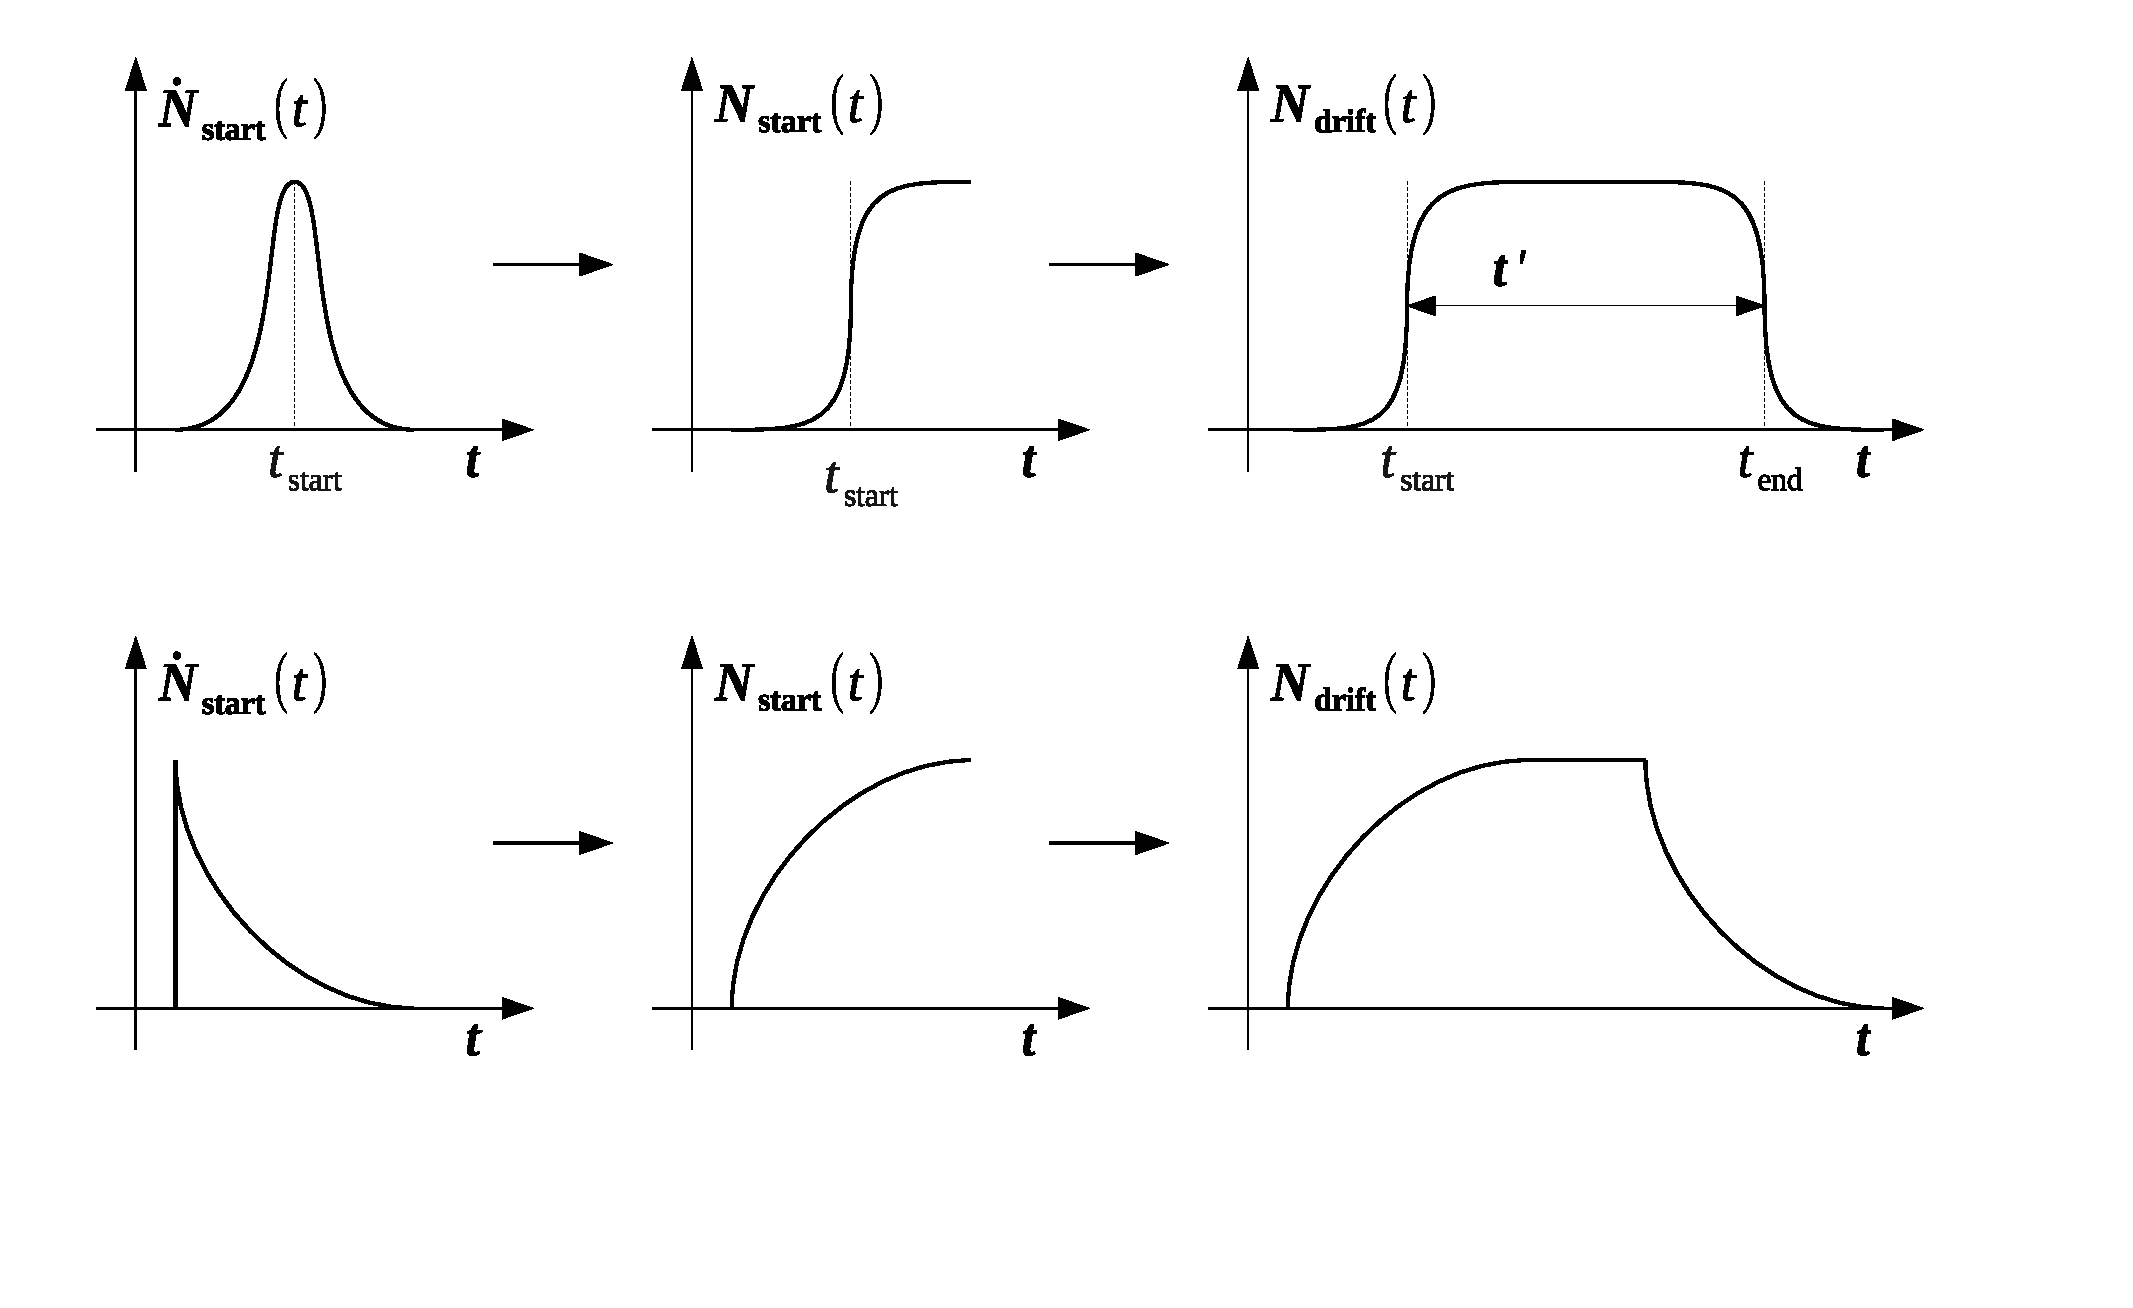
\includegraphics[trim=0cm 3cm 3.5cm 0cm, clip=true,width=0.79\textwidth]{figures/driftingcharges2.eps}
\put(-380,175){(A)}
\put(-380,69){(B)}
 \caption{\textbf{(A)} A Gaussian and \textbf{(B)} an exponential start time distribution function \textbf{(left column)},
 their resulting number of started charges distribution function \textbf{(middle column)}
 and the drifting charges distribution \textbf{(right column)} are shown.}
 \label{fig:collection}
\end{figure}


\subsection{Total integrated current}

\begin{figure}[tb]
 \centering
 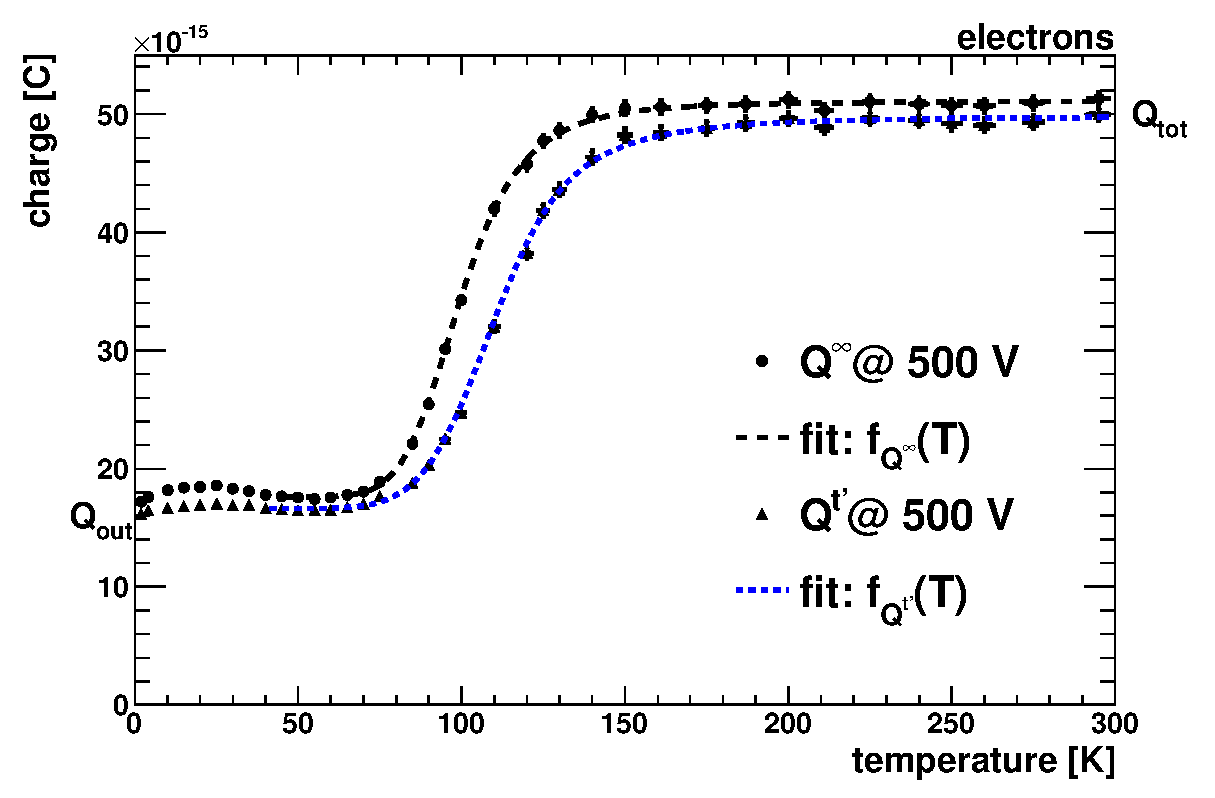
\includegraphics[width=0.49\textwidth]{figures/QttrTmultiE_e.eps}\put(-180,110){\LARGE (A)}\vspace{0.3cm}
 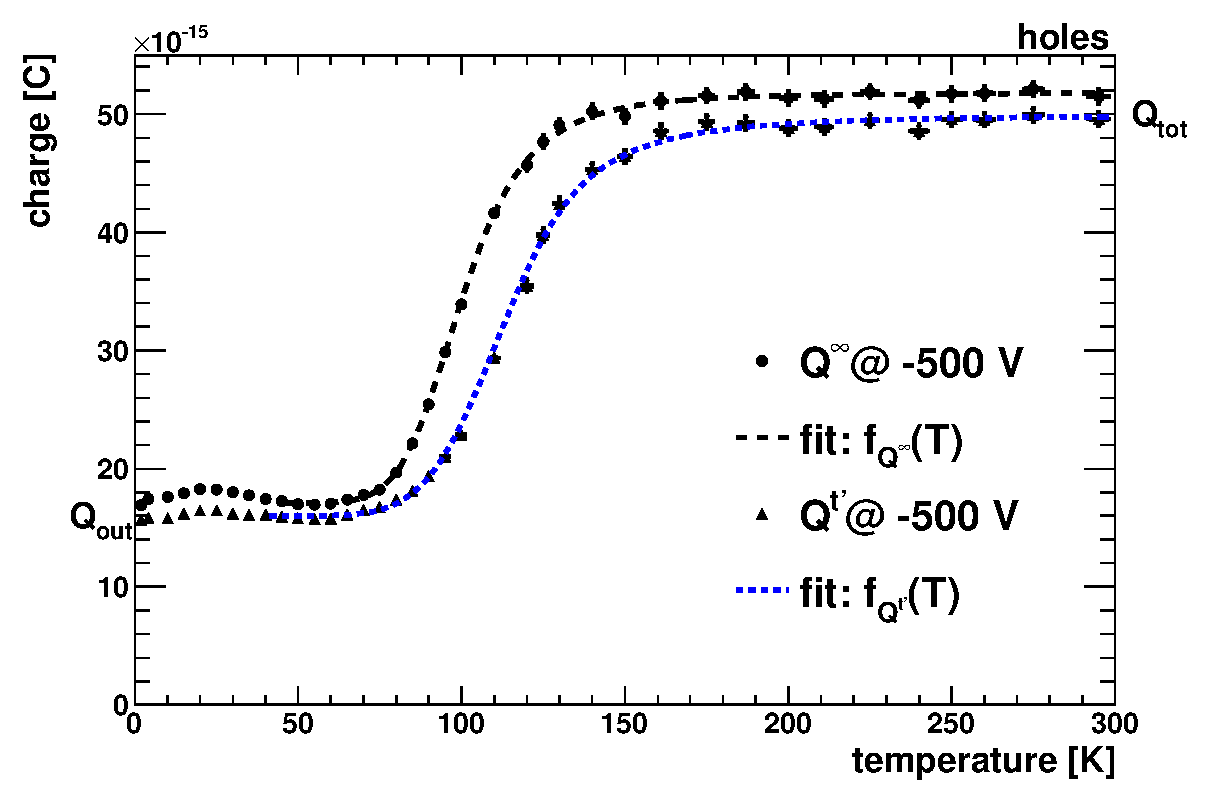
\includegraphics[width=0.49\textwidth]{figures/QttrTmultiE_h.eps}\put(-180,110){\LARGE (B)}
 \caption{The measured charge as a function of the temperature is shown for $Q^{\textrm{|infty}}$ and $Q^{t'}$ for \textbf{(A)} electrons and \textbf{(B)} holes.}
 \label{fig:QT}
\end{figure}

The measured current is integrated over time and analysed as a function of temperature, which is shown in 
 Fig.~\ref{fig:QT} for electrons \textbf{(A)} and holes \textbf{(B)} at $E \approx \SI{1}{\volt/\micro\meter}$, or an applied voltage of $\SI{500}{\volt}$. 
An S-curve describes the overall shape of the measured charge. 
Two variations of the collected charge are shown, the upper one, $Q^{\infty}$, integrates the current including the exponentially falling tail,
 the lower one, $Q^{t'}$ integrates up to the transit time omitting the tails. 
The statistical uncertainty on the charge is estimated to be around 1\,\%. 
The integral of the current pulses is constant at about $Q = \SI{52.0(5)}{\femto\coulomb}$ between room temperature and $\SI{150}{\kelvin}$,
 decreases to about one third of the RT value towards $\sim$ $\SI{75}{\kelvin}$, and remains at this level towards even lower temperatures.
The fit-function, justified in section~\ref{sec:discussion}, contains four parameters: (1) the total charge, (2) the \textit{outer} charge, cf.\ section~4, and (3) a factor $\varepsilon$ in combination with a
 Boltzmann factor 
 with (4) an activation energy $\Ea$. 
The total charge $\Qtot$ and the outer charge $\Qo$ are highly predetermined by the two plateaus before and after the charge drop at about 52\,fC and 17\,fC, respectively, 
 and the inner charge is then $\Qin = \Qtot - \Qo$. 
The fit function for the measured charge $Q^{\infty}$ becomes

\begin{equation}
 f_{Q^{\infty}}(T) = \Qo + \frac{\Qin}{1+\varepsilon\cdot\exppEa},\phantom{\frac{\tau}{\ttr}\exp{\left(-\ttr/\tau\right)}}.
 \label{eq:fitQinfty}
\end{equation}

The fit-function for $Q^{t'}$ is more complicated, as it involves the transit time $\ttr$ and the shape constant $\tau$. 
Therefore, it contains five free parameters ($\Qtot$, $\Qo$, $\varepsilon$, $\Ea$, $\tau$). %, again with $\Qtot$ and $\Qo$ highly predetermined. 
$\ttr$ is taken from data, cf. section~\ref{sec:tt},
 i.e.~a simple power law fit of the transit time as a function of the temperature at $E \approx \SI{1}{\volt/\micro\meter}$. 
The fit-function then reads

\begin{equation}
 f_{Q^{t'}}(T) = \Qo + \frac{\Qin}{1+\varepsilon\cdot\exppEa}\cdot \frac{\tau}{\ttr} \cdot \left[ 1 - \frac{\tau}{\ttr} (1 - \exp{\left(-\ttr/\tau\right)}  ) \right] ,
 \label{eq:fitQtprime}
\end{equation}

\noindent
with a shape constant $\tau$ describing the exponential flanks. 

\begin{table}[tb]
 \centering
 \caption{The results of fitting, firstly, Eq.~(\ref{eq:fitQtprime}) to the charge collected until $\ttr$ ($Q^{t'}$, i.e.~without the tail)
 and secondly Eq.~(\ref{eq:fitQinfty}) to the charge including the tail ($Q^{\infty}$) are listed for electrons and holes at a bias voltage of 500\,V. {\color{red}(A3)}}
   \vspace{0.5cm}

 \begin{tabular}{lcccccc}
\toprule
 & \multicolumn{6}{c}{$Q^{t'}$}  \\  \midrule% \cmidrule(r){2-6} \cmidrule(l){7-10}
 & $\Qtot$\,[fC] & $\Qo$\,[fC] & $t_{e,0}$\,[ps] &  $\taurec$\,[ns]  & $\Ea$\,[meV]& $\chi^2/\textrm{ndf}$\\
% &  fixed	 &  free       & free  &  free     &                             & fixed         & free        & free                           & \\
\midrule
 $\e$ & $\num{49.8(2)}$ & $\num{16.6(3)}$ & $\num{0.6(2)}$ & $\num{14}$ (fixed) & $\num{79(3)}$ & 0.9 \\
 $\h$ & $\num{50.0(2)}$ & $\num{16.0(3)}$ & $\num{1.1(3)}$ & $\num{14}$ (fixed) & $\num{76(3)}$ & 1.4 \\ \midrule
 & \multicolumn{6}{c}{$Q^{\infty}$}\\ \midrule
 & $\Qtot$\,[fC]   & $\Qo$\,[fC]     &  $\num{e5}\,\varepsilon$  & & $\Ea$\,[meV] & $\chi^2/\textrm{ndf}$ \\ 
 \midrule
$\e$ & $\num{51.1(2)}$ & $\num{17.6(3)}$ & $\num{2.8(9)}$     & & $\num{90(3)}$ & 0.4\\
$\h$ & $\num{51.8(2)}$ & $\num{17.1(3)}$ & $\num{5.1(15)}$    & & $\num{85(3)}$ & 0.5\\
avg  & 51.5            & 17.4            & $\num{3.4(8)}$     & & $\num{87.5(22)}$ & \\
\bottomrule
 \end{tabular}
 \label{tab:fitQ}
\end{table} %FIXME re-fit, paste values

{\color{red}(A2)} [The result of the fits for $Q^{t'}$ and $Q^{\infty}$ are tabulated in Tab.~\ref{tab:fitQ} for both carrier types
 and the fit-functions are superimposed as dotted lines in Fig~\ref{fig:QT}. 
The inner charge constitutes about 2/3 of the total charge at a field of $E = \SI{1}{\volt/\micro\meter}$, the outer charge about 1/3,
 summing to a total of about 52\,fC. 
Estimates of $t_{e,0}$ and $\taurec$ are obtained by the following consideration. 
At around 100\,K, $\Qin$ has decreased to half of its RT value, see Fig.~\ref{fig:QT}. 
Therefore $\frac{1}{1+\frac{\tauevap}{\taurec}} = \frac{1}{2}$ and hence $\tauevap = \taurec$. 
With a measured shape constant of $\SI{7}{\ns}$ at 100\,K, cf.\ section~3.5, both the recombination lifetime and the evaporation time at 100\,K are $\sim$ $\SI{14(2)}{\ns}$,
 and therefore $\tauevap = t_{e,0} \exppEa \approx \SI{14}{\ns}$.
Thus, $t_{e,0}$ becomes 

\begin{equation}
 t_{e,0} = \SI{14(2)}{\ns} / \exp{\big( \SI{0.0875}{\eV}/(\kB\cdot \SI{100}{\kelvin}) \big)} = \SI{0.5(1)}{\ps}.
\end{equation}

\noindent
(!) The fit $f_{Q^{t'}}$ does not converge for $\taurec$, we therefore fixed $\taurec$ at a reasonable value of $\taurec = \SI{14}{\ns}$. 
Then, the fit yields
\begin{equation}
 t_{e,0} = \SI{0.6(2)}{ps}
\end{equation}
 
\noindent
in reasonable accordance with the earlier evaluated $t_{e,0}$-value.  
A third estimation results from the $Q^{\infty}$-fit (Eq.~(\ref{eq:fitQinfty})), where only the ratio $\varepsilon = t_{e,0}/\taurec$ appears:
\begin{equation}
 \varepsilon = t_0/\taurec = (\num{3.4(8)})\,\num{e-5}
\end{equation} 

\noindent
averaging the results from electrons and holes, see Tab.~\ref{tab:fitQ}. 
Using again the evaporation time $\tauevap \approx \SI{14(2)}{\ns}$, it is found that

\begin{equation}
 t_{e,0} = \SI{14(2)}{\ns} \cdot \varepsilon = \SI{0.5(2)}{\ps}.
\end{equation}

\noindent
With $t_{e,0} \approx \SI{0.5}{\ps}$, the evaporation time at 50\,K, 150\,K and 300\,K follow to be of the order of $\SI{600}{\micro\second}$, $\SI{600}{\micro\second}$ and $\SI{30}{\ps}$, respectively. 
It is emphasised that the experimentally found scale of $t_{e,0}$ is crucial for the description of the observed data.
If $t_{e,0}$ was of the order of femtoseconds, the charge would not have decreased to half of its RT value at 100\,K, but at 58\,K. 
Also, the rise time of the current pulse at 150\,K would have increased to ??, which is experimentally not observed. 
In the same manner, activation energies of the order of 40\,meV are strictly excluded. 
]

\begin{figure}[tb]
 \centering
 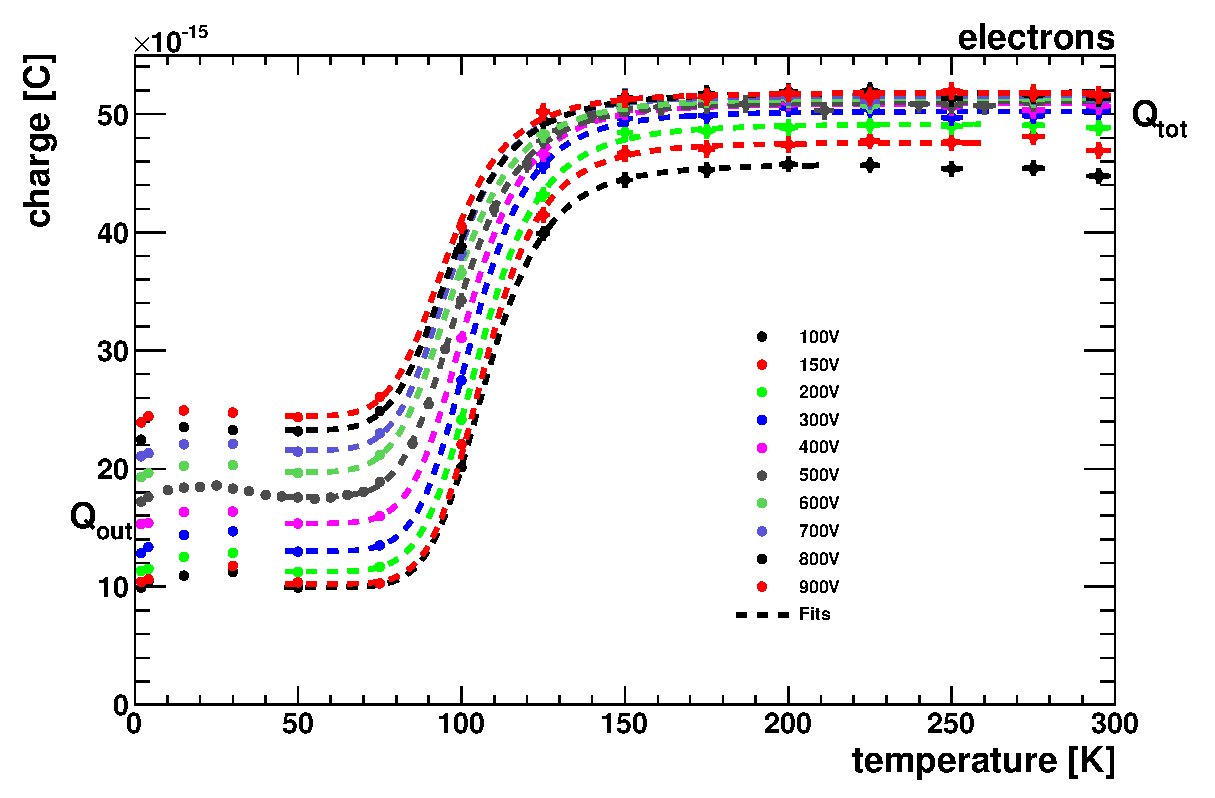
\includegraphics[width=0.49\textwidth]{figures/QTmultiE_e.eps}\put(-180,120){(A)}\vspace{0.3cm}
 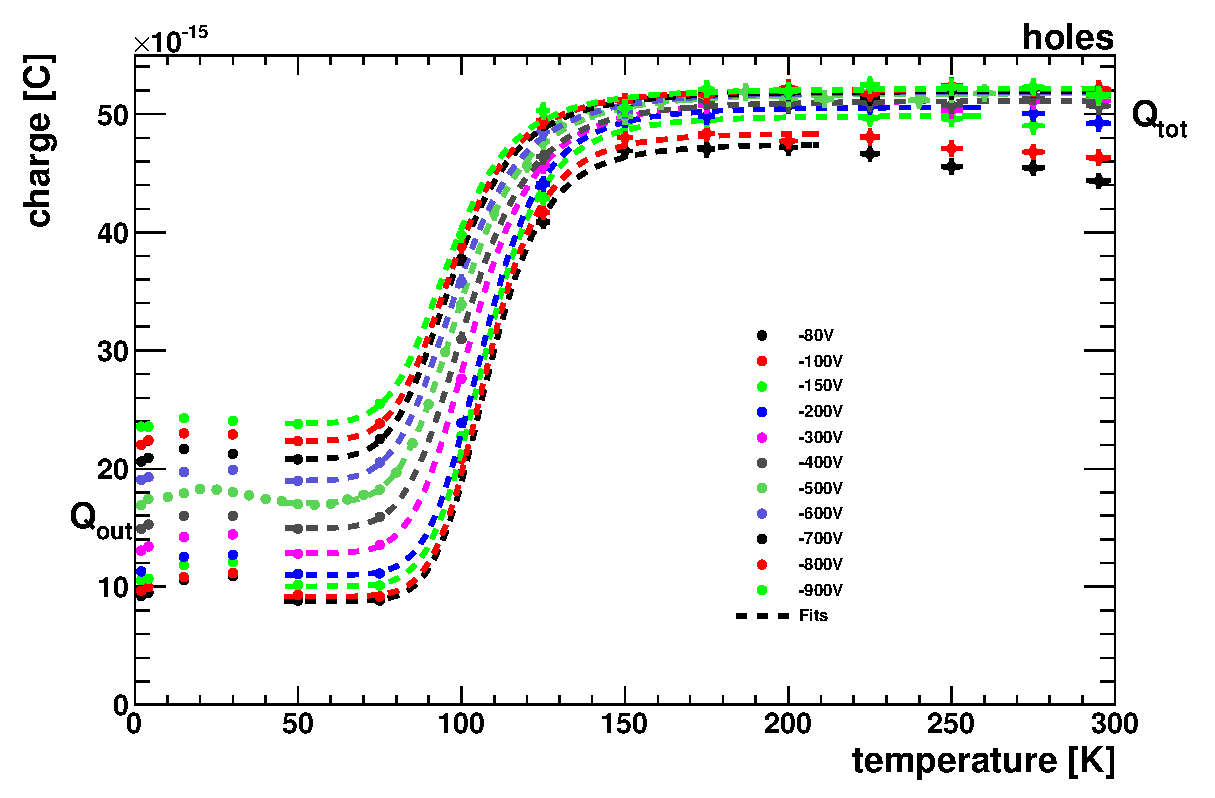
\includegraphics[width=0.49\textwidth]{figures/QTmultiE_h.eps}\put(-180,120){(B)}
 \caption{The measured charge $Q^{\infty}$ as a function of the temperature is shown for various voltages for electrons \textbf{(A)} and holes \textbf{(B)}.}
 \label{fig:QTvoltage}
\end{figure}

The S-curves for different voltages are shown for $Q^{\infty}$ in Fig.~\ref{fig:QTvoltage}. 
Again, the similarity between electron and hole pulses is evident. 
The fit described earlier is performed for charge data from 100\,V to 900\,V, each fit resulting in a value for $\varepsilon$, and $\Ea$. 
The discussion of the temperature dependence of the fit-parameters ist postponed to section~\ref{sec:discussion}. 

\begin{figure}[tb]
 \centering
 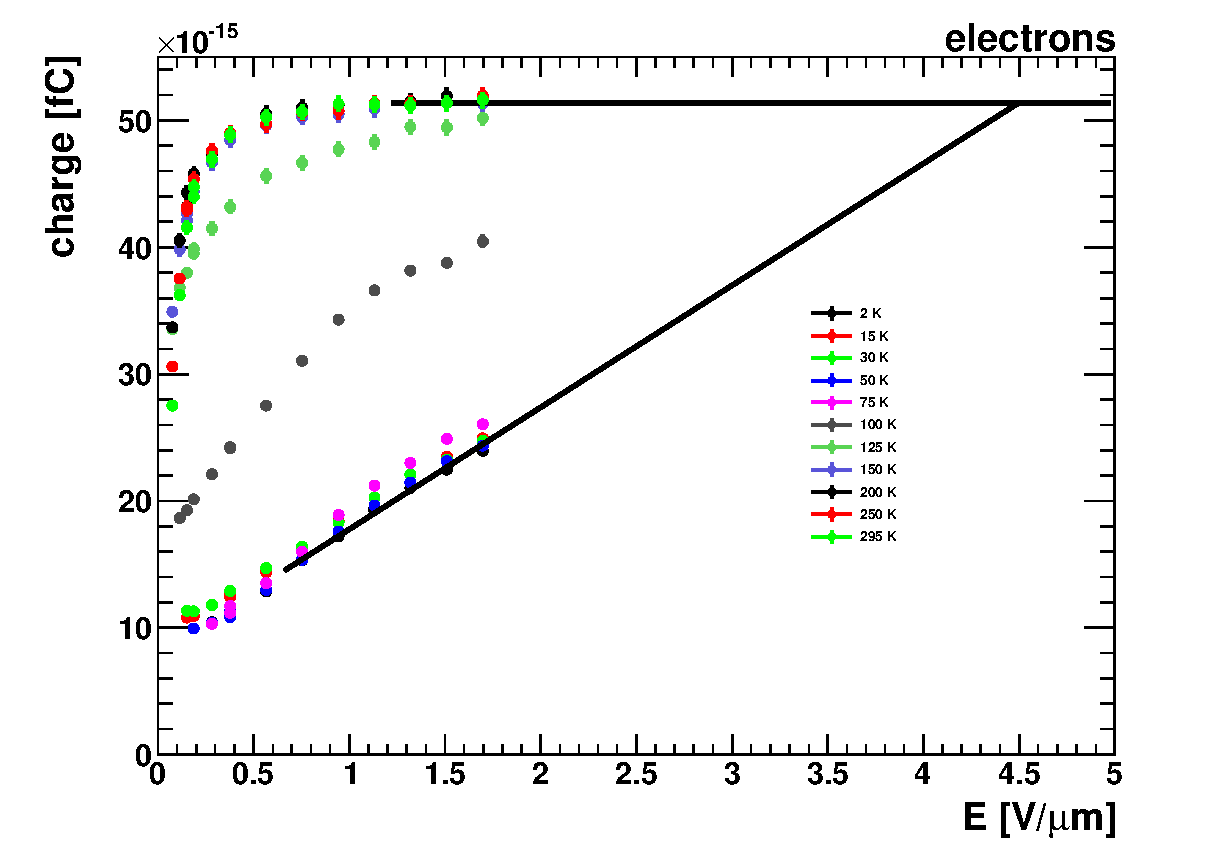
\includegraphics[width=0.49\textwidth]{figures/QEmulti_e}\put(-180,120){(A)}\vspace{0.3cm}
 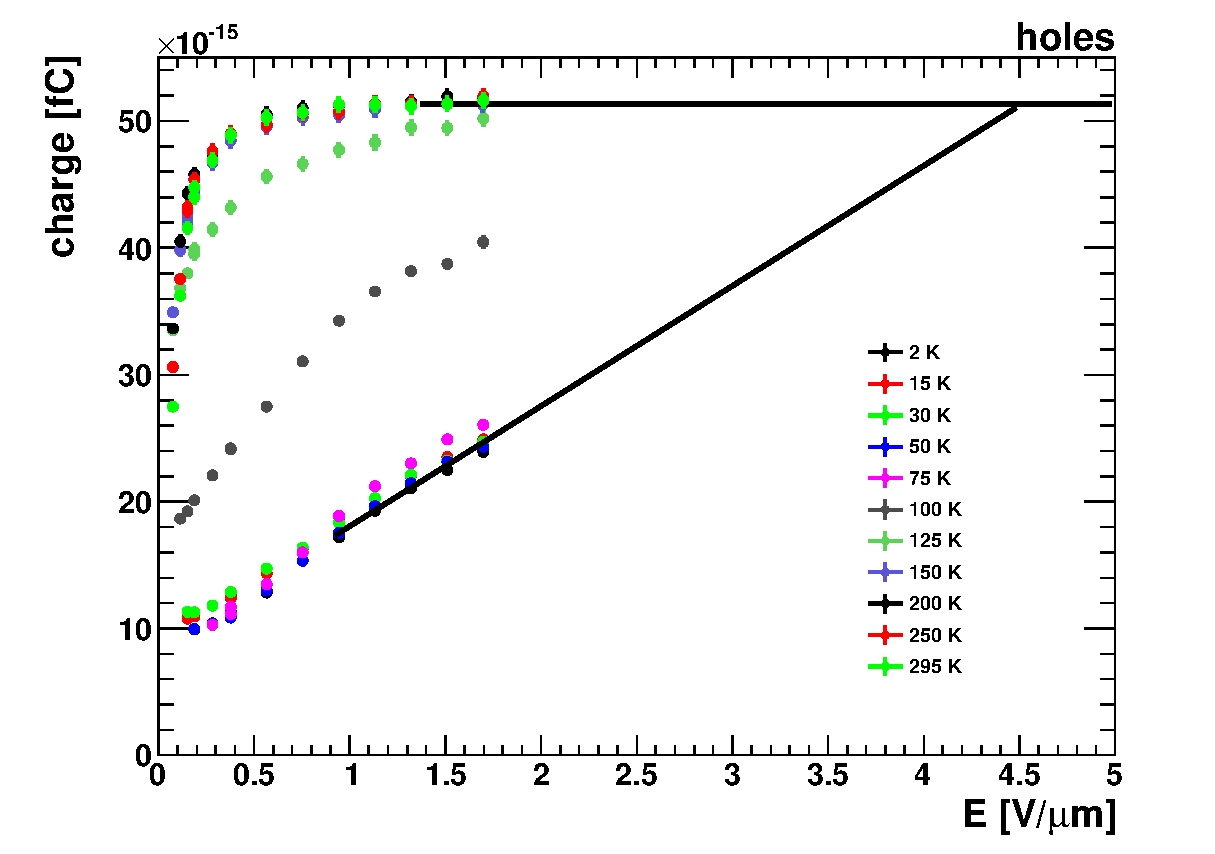
\includegraphics[width=0.49\textwidth]{figures/QEmulti_h}\put(-180,120){(B)}
 \caption{The measured charge $Q^{\infty}$ as a function of the applied field strength is shown for various temperatures for electrons \textbf{(A)} and holes \textbf{(B)}.}
 \label{fig:QvsE}
\end{figure}

Plotted as a function of the electric field strength, the influence of the field on the measured charge becomes evident.
Figure~\ref{fig:QvsE} shows the same behaviour for all temperatures above 150\,K, and below 75\,K. 
The first increases rapidly with field strength and reaches a flat top at about $\SI{1}{\volt/\micro\meter}$, whereas the latter increases linearly. 
The discussion of this behaviour is covered in section~4. 

\subsection{Fit-function for the current pulses}

The transit time and characteristic time constant are determined by the time difference between end time and start time of drift,
 $t_{\text{e}}$ and $t_{\text{s}}$ respectively, hence $\ttr = t_{\text{e}} - t_{\text{s}}$.
A function $f(t;P)$ is fitted to each current pulse in order to find $t_{\text{e}}$ and $t_{\text{s}}$.
$f(t;P)$ is a function of time and a set of parameters $P$ incorporating two complementary error functions $(2-\Erfc(t-t_{\text{s}}))$ and $\Erfc(t-t_{\text{e}})$
 describing the rising and the falling edge, respectively. 
Additionally, an exponential component  of the form $\left( 1-\exp \left(-(t-t_{\text{s}})/\tau\right) \right) - \Theta_{\textrm{col}}(t;t_{\text{e}})$ with
  $\Theta_{\textrm{col}}(t;t_{\text{e}}) = 1 - \exp \left( -(t-t_{\text{e}})/\tau \right)$ for $t > t_{\text{e}}$ and $\Theta_{\textrm{col}}(t;t_{\text{e}}) = 0$ otherwise,
 is allowed, cf.~Eq.~(\ref{eq:collection}). 
The error functions describe a Gaussian probability distribution for the start time of the drift around $t_{\text{s}}$,
 and respectively a collection at the opposite electrode around $t_{\text{e}}$. 
The 50\% points mark $t_{\text{s}}$ and $t_{\text{e}}$, respectively. 
The fit parameter $\tau$ is given a physical meaning in the discussion section. 

At all temperatures and fields, the fit-function describes well the measured pulse shape of $i_m(t)$;
 each fit resulting in a value for $\tau(T,E)$ and $\ttrans(E,T)$.
One example of a fit to a measured pulse $i_m(t)$ at 100\,K and 500\,V is shown in Fig.~\ref{fig:ExModel2}. 
The resulting shape constant is $\tau(\SI{100}{\kelvin},\,\SI{500}{\volt}) \approx (\num{6.8}\pm\num{0.1}_{\textrm{stat}}\pm\num{1.0}_{\textrm{sys}})\,\si{\ns} \approx \SI{7(1)}{\ns}$. 
The current induced from charges stemming from the outer and the inner part of the cloud are shown separately as dashed lines
 featuring the error-function shape and the exponential shape, respectively.
The sum forms the solid line on top of the data. 
At this temperature, a certain fraction of the charge recombines. 

\subsection{Characteristic time constant}

\begin{figure}[t]
 \centering
 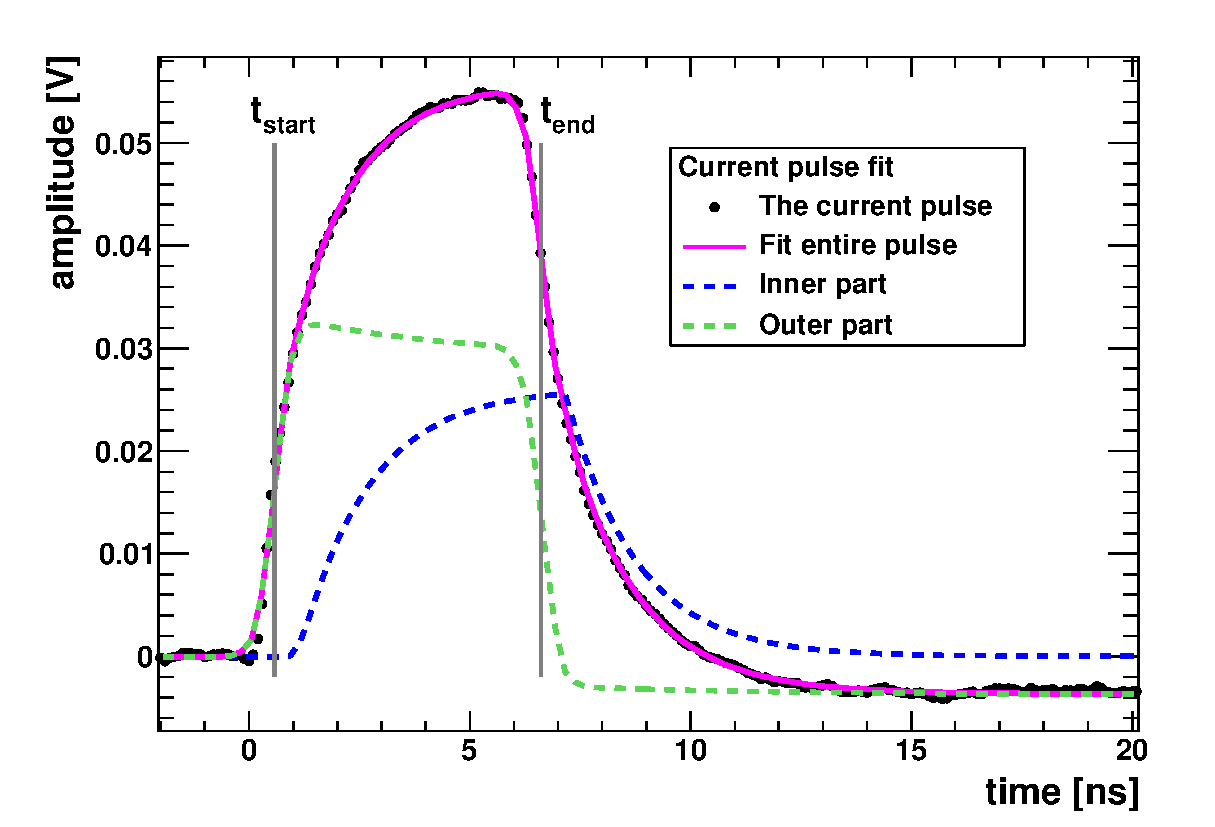
\includegraphics[width=0.59\textwidth]{figures/ex_pulsefit3}%pulseFit.C
 \caption{The fit to the measured pulse at 100\,K and 500\,V and its components are depicted.}
 \label{fig:ExModel2}
\end{figure}


The fitted shape constant $\tau$ is shown in Fig.~\ref{fig:fittau}
 as a function of temperature (closed circles) at $E \approx \SI{1}{\volt/\micro\meter}$. 
The error bars are the statistical errors resulting from the fit. 
For both electrons and holes $\tau$ remains about constant at $\SI{0.4}{\ns}$ between RT and $\SI{150}{\kelvin}$. 
Between $\SI{150}{\kelvin}$ and $\SI{90}{\kelvin}$, the shape constant increases steeply.%
\footnote{A comparison to measured values in the literature is difficult, or impossible,
 as no measurement of exciton properties in diamond using electric fields are known to the authors.}
Due to the decrease of the amplitude of the tail in the current pulses with decreasing temperature, the signal-to-noise ratio at $T \leq \SI{90}{\kelvin}$
 is too small in order to accurately fit the shape constant. 
The fitted $\tau$ therefore decreases for $T < \SI{90}{\kelvin}$. 
The corresponding region is marked as `insensitive'. 

\begin{figure}[t]
 \centering
  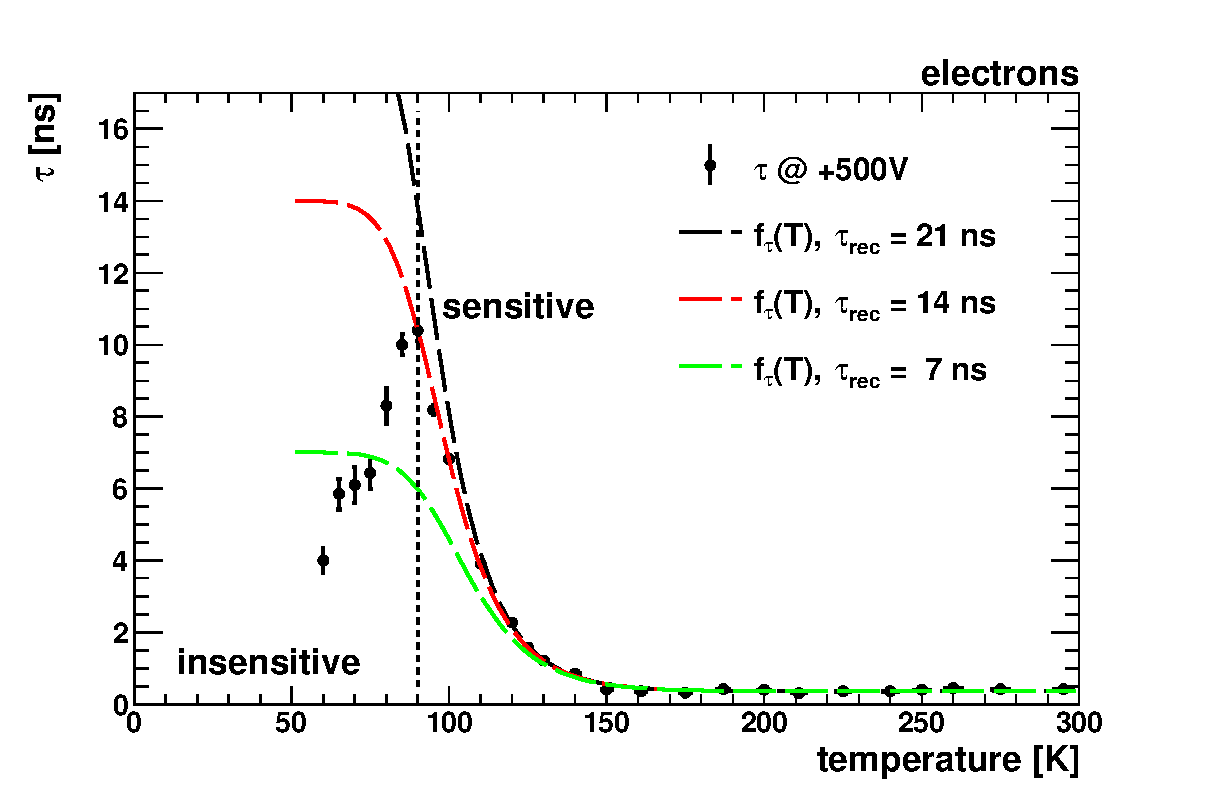
\includegraphics[width=0.49\textwidth]{figures/tauvsT_e}\put(-190,110){(A)}
  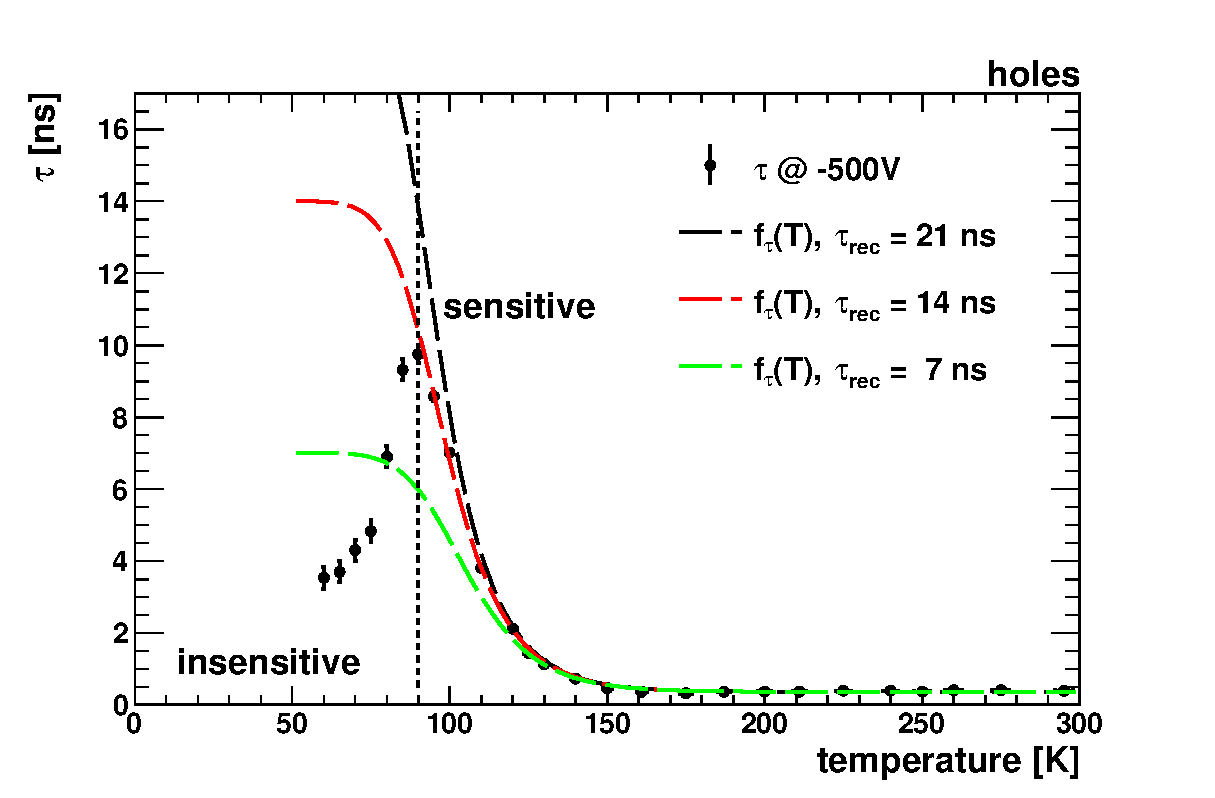
\includegraphics[width=0.49\textwidth]{figures/tauvsT_h}\put(-190,110){(B)}\\
  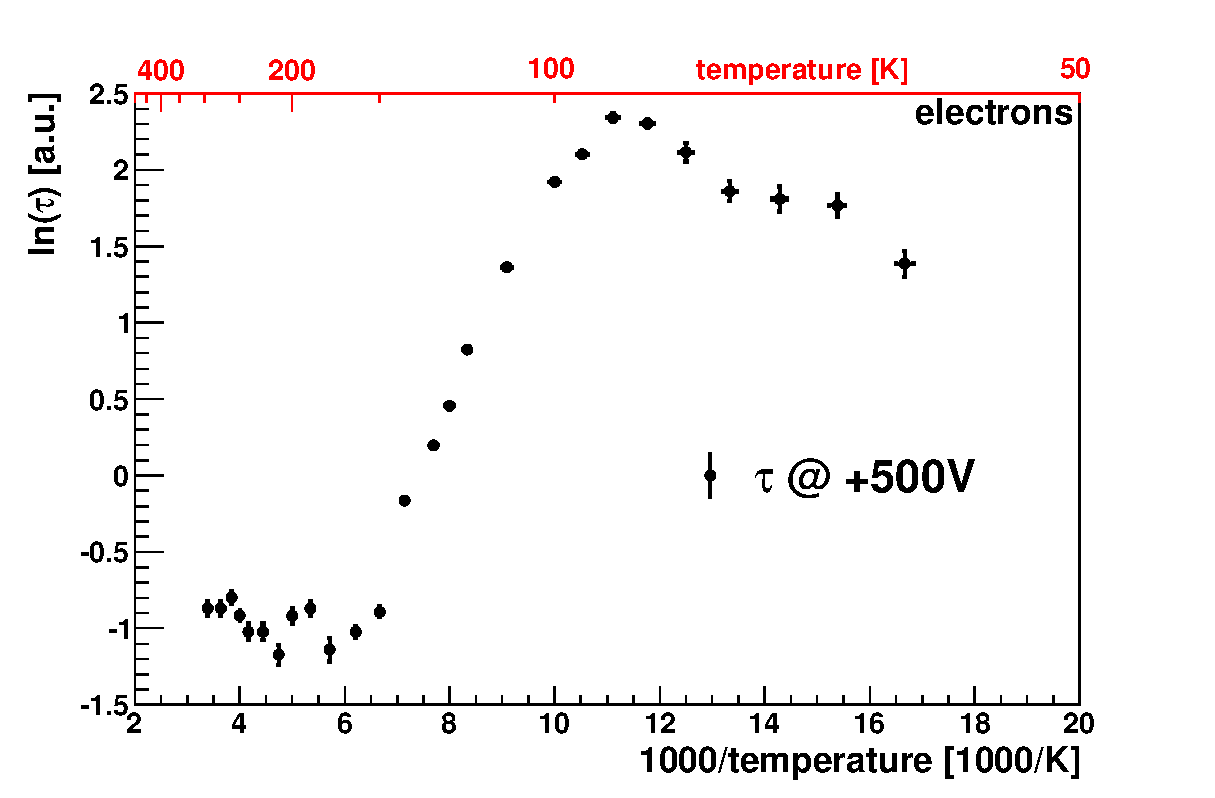
\includegraphics[width=0.49\textwidth]{figures/logtauvsTinv_e}\put(-190,110){(C)}
  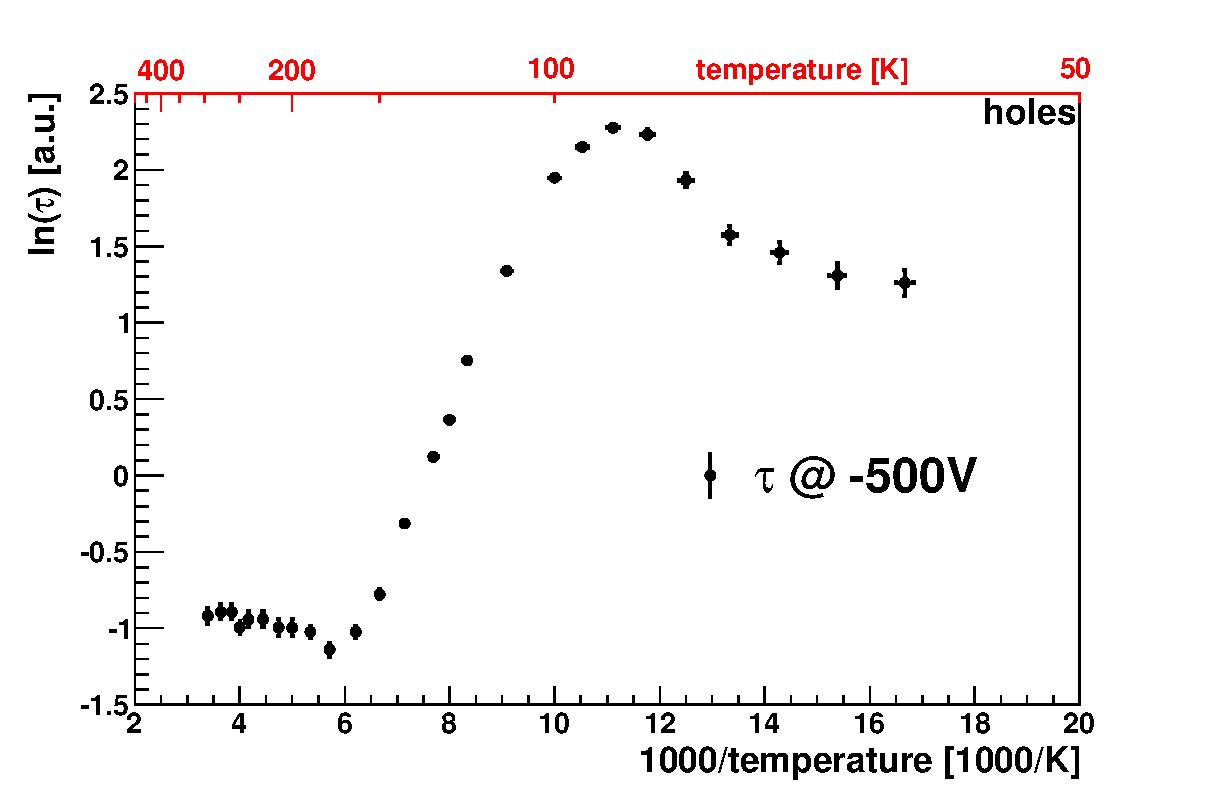
\includegraphics[width=0.49\textwidth]{figures/logtauvsTinv_h}\put(-190,110){(D)}
 \caption{The fitted shape constant $\tau$ is shown as a function of the temperature for electrons \textbf{(A)} and holes \textbf{(B)} at $500$\,V.
\textbf{(C)} and \textbf{(D)} show the results in $\ln{(\tau)}$ vs.~the inverse temperature.}
 \label{fig:fittau}
\end{figure} %FIXME title x-axis = 1000/temperature

We revise, if the measured temperature dependence of $\tau$ can be explained within the exciton model
 using the $t_{e,0}$-value (0.5\,ps) extracted from charge data. 
Using $\frac{1}{\tauzero} =  \frac{1}{\taurec} + \frac{1}{\tauevap}$ and $\tauevap = t_{e,0} \exppEx$ one finds

\begin{equation}
 \tauzero(T) = \left( \frac{1}{\taurec} + \frac{1}{\tauevap(T)} \right)^{-1} = \left( \frac{1}{\taurec} + \frac{1}{t_{e,0} \exppEx }\right)^{-1}.
 \label{eq:tauT}
\end{equation}

\noindent
A possible temperature dependence of the recombination lifetime is not allowed for. 
It is further important to notice that
 the fitted shape constant cannot be faster than the cut-off time constant, which arises from the cut-off frequency of the measuring system. 
In fact, the cut-off constant adds quadratically to the physical shape constant, resulting in the fitted shape constant.
Using Eq.~(\ref{eq:tauT}) and an additional such parameter $\tau_{cut}$, a function $f_{\tau}(T)$ is defined  as

\begin{equation}
 f_{\tau}(T) = \sqrt{\left( \frac{1}{\taurec} + \frac{1}{t_{e,0} \exppEx }\right)^{-2} + \left( \tau_{\textrm{cut}}\right)^2},
 \label{eq:fittau}
\end{equation}

\noindent
which is to be checked against the data. 
Superimposed in Fig.~\ref{fig:fittau} as dashed lines are $f_{\tau}(T)$ with the activation energy $\Ea = \SI{87.5}{\milli\eV}$, $t_{e,0} = \SI{0.5}{\ps}$,
 and three different $\taurec = 7,14,\SI{21}{\nano\second}$. 
It is clear from Fig.~\ref{fig:fittau} that Eq.~(\ref{eq:fittau}) describes the experimental data reasonably well
 using the afore mentioned $\Ea(\SI{500}{\volt}) = \SI{87.5}{\milli\eV}$, $t_{e,0} = \SI{0.5}{\ps}$, and $\taurec = \SI{14}{\ns}$. 
Therefore, a combination of values $\Ex$ and $t_{e,0}$ exists that consistently explains two important parts of the data,
 i.e.~the temperature dependence of both the measured charge and the fitted shape. 

The characteristic time constant shall also be studied as a function of the temperature in order to extract the activation energy as a function of the electric field. 

\begin{figure}[t]
 \centering
  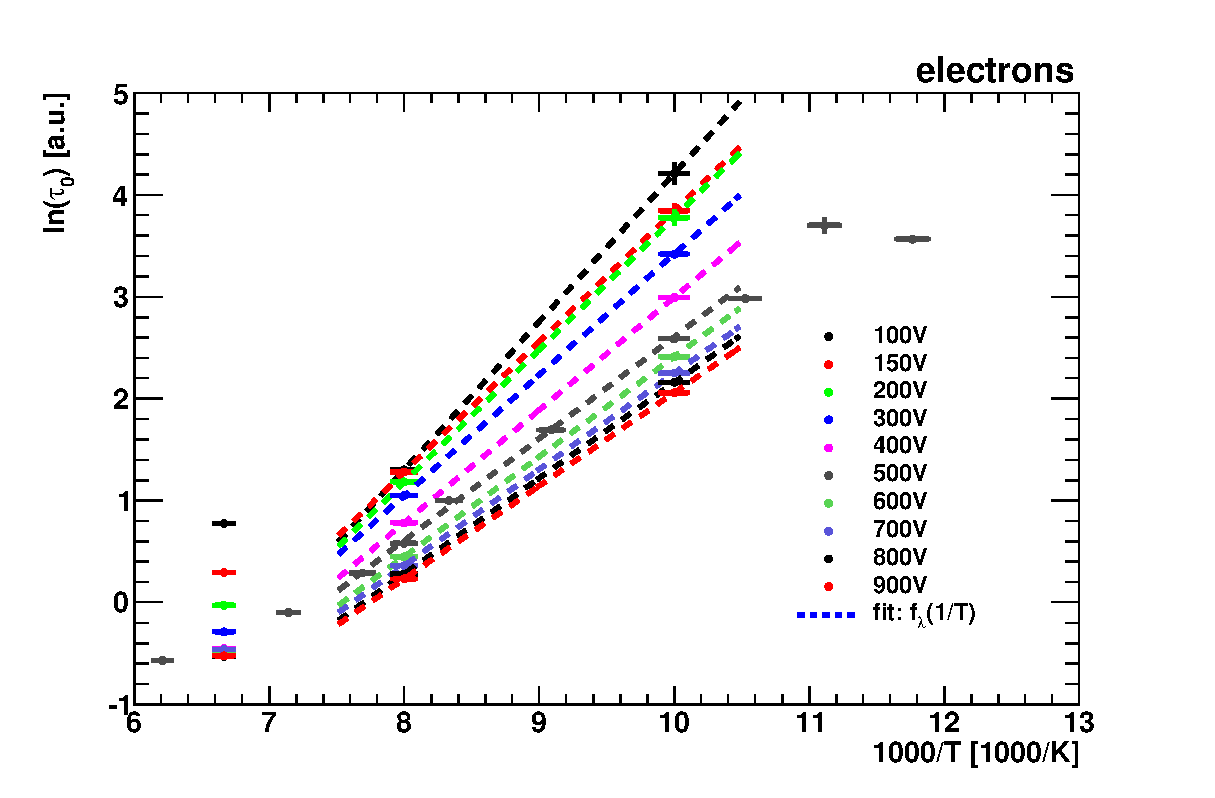
\includegraphics[width=0.49\textwidth]{figures/logtauvsTinvU_e}\put(-190,110){(A)}
  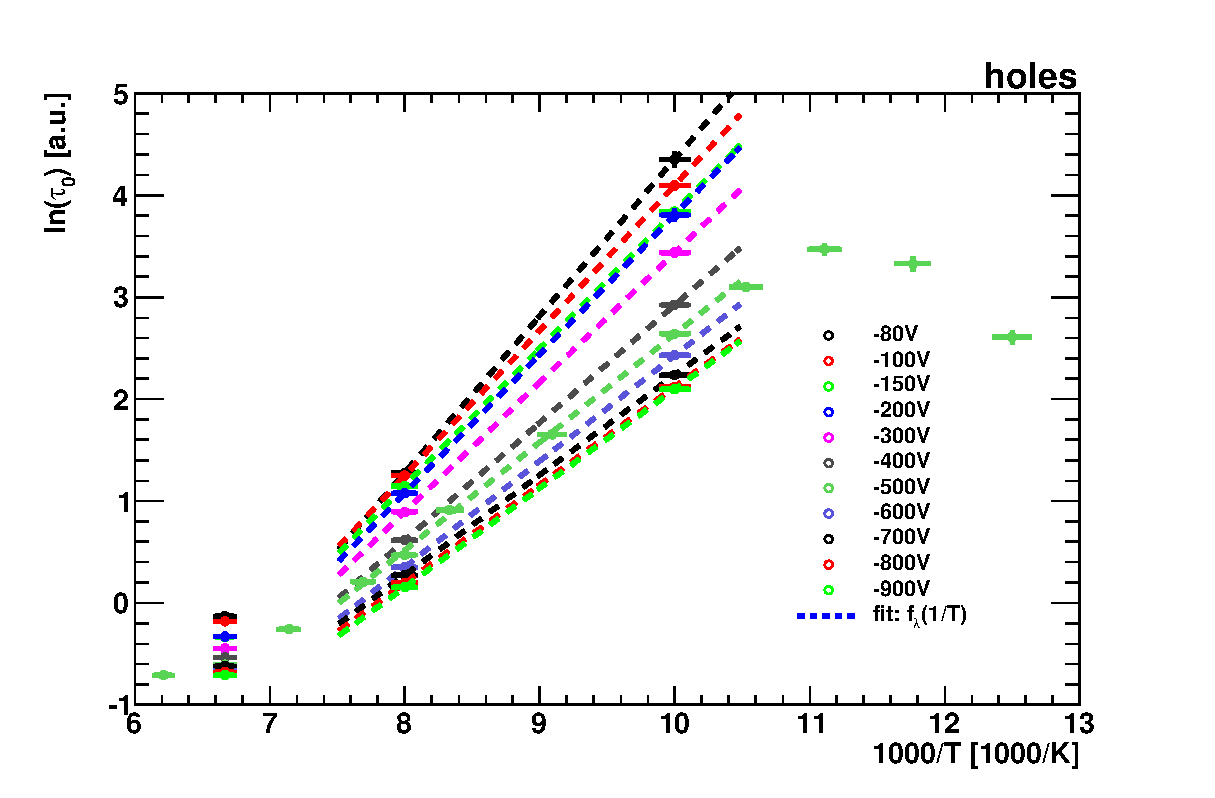
\includegraphics[width=0.49\textwidth]{figures/logtauvsTinvU_h}\put(-190,110){(B)}
 \caption{The fitted shape constant is shown as $\ln{(\tauzero)}$ versus the inverse temperature for various voltages including their corresponding linear fits extracting the activation energy. }
 \label{fig:fittauV}
\end{figure}

\subsection{Transit time}
\label{sec:tt}

\begin{figure}[t]
 \centering
 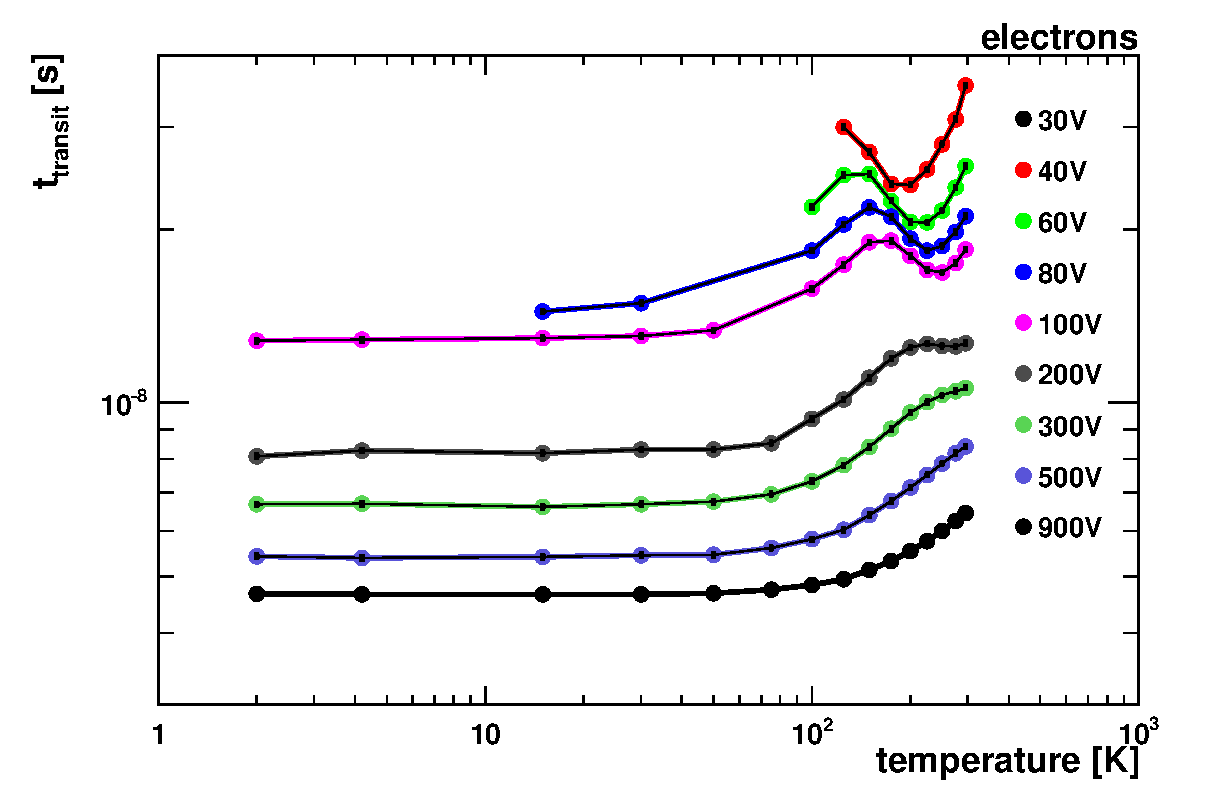
\includegraphics[width=0.49\textwidth]{figures/ttloglog_e.eps}\put(-190,110){(A)}
 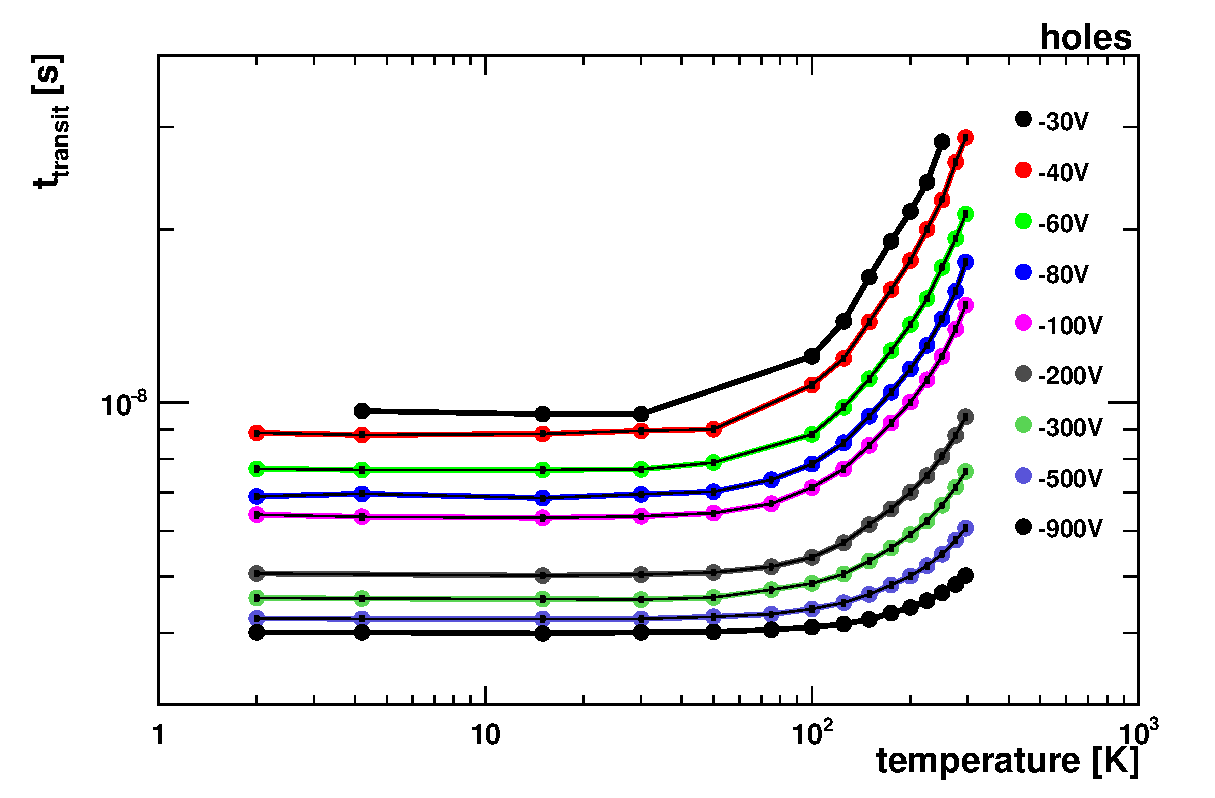
\includegraphics[width=0.49\textwidth]{figures/ttloglog_h.eps}\put(-190,110){(B)}
 

 \caption{The transit times for holes \textbf{(a)} and electrons \textbf{(b)} at various temperatures and fields are shown for \textit{S57}. 
Note the double logarithmic scale. Lines are drawn between measurements for constant voltages in order to guide the eye.}
 \label{fig:tt}
\end{figure}

The measured transit times are shown in Fig.~\ref{fig:tt} for \textit{S57} as an example. 
All three samples show the same behaviour. 
Transit times range from $\SI{3}{\nano\second}$ to $\SI{40}{\nano\second}$ for all fields and temperatures. 
Experimental sources of uncertainties affecting the measurement of the drift velocity are listed below including an estimate of their values.
\begin{itemize}
 \item[1)] The sample thickness has been measured with precision tools resulting in an uncertainty of the sample thickness below $<1\%$.
 \item[2)] The error in the measurement of the transit time $\sigma_{\ttr}$ depends on the ability to identify the rising and the falling edge, which in turn correlates with the SNR.
The SNR depends on the temperature and the electric field. 
$\sigma_{\ttr}$ is estimated as $\sigma_{\ttr} = \frac{\sigma_{\textrm{noise}}}{\textrm{slope}}$, with the baseline noise $sigma_{\textrm{noise}}$ and the maximum slope in the rising edge. 
At room temperature (low temperature) and $E\approx \SI{1}{\volt/\micro\meter}$, this approach leads to uncertainties of the transit time measurement of around $1\%$ ($2\%$),
 and up to $4\%$ at low temperature and low fields.
 \item[3)] At low SNRs the bandwidth limit was used in order to extent the accessible measurement range towards lower electric fields. 
The bandwidth limit leads to slower rising and falling edges. 
The effect on the transit time at $V_{\textrm{bias}} = \SI{100}{\volt}$ at RT is $\approx1\,\%$. 
At lower biases the rising/falling edges are slower, hence the effect is smaller. 
 \item[4)] Errors due to a possible non-uniformity of the electric field can be neglected, as a net-space charge seems to be absent in the tested samples.
 \item[5)] The uncertainty of the electric field strength is conservatively estimated to $1\%$.
 \item[6)] The uncertainty of the temperature measurement is about $1\%$. 
\end{itemize}




Figure~\ref{fig:tt} (a) shows how the transit time for holes increases with temperature over the entire temperature range,
 and how it decreases with increasing field over the whole field range. 
For electrons, Fig.~\ref{fig:tt} (b), the transit time decreases with increasing field, but does not monotonically increase for all biases. 
Only at high biases, down to $\SI{300}{\volt}$, the transit time increases with increasing temperature over the whole temperature range.
For smaller biases, a local maximum emerges, being more pronounced with decreasing bias.
The position of the local maximum shifts to lower temperatures with decreasing bias.
The abnormal behaviour of the electron transit time is likely to be caused by a re-population effect, a well-understood phenomenon in silicon \cite{Jacoboni197777}.
It was recently observed in high-purity scCVD diamond \cite{isberg:172103}, but at much lower temperatures and fields. 

 
